\documentclass[convert]{standalone}

\usepackage{tikz}
\usepackage{graphicx}
\pagestyle{empty}

% INT_AY22_L28-Fig05_Disp_current_cap.png

\begin{document}
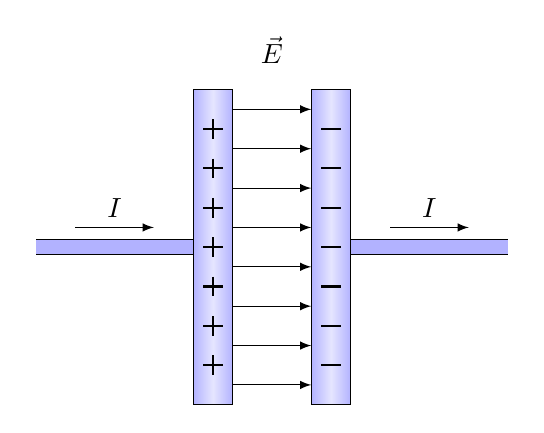
\begin{tikzpicture}[> = latex]
	
	% Wires connecting plates w currents
	
	\draw [double = blue!30, double distance = 5 pt] (-1, 0) -- (-3, 0);
	\draw [->] (-2.5, 0.25) -- node [above] {$I$} (-1.5, 0.25);
	
	\draw [double = blue!30, double distance = 5 pt] (1, 0) -- (3, 0);
	\draw [->] (1.5, 0.25) -- node [above] {$I$} (2.5, 0.25);

	% Capacitor plates w charges
	
	\draw [left color = blue!30, right color = blue!30, middle color = blue!10] (-1, -2) rectangle (-0.5, 2);
	\draw [left color = blue!30, right color = blue!30, middle color = blue!10] (1, -2) rectangle (0.5, 2);
	
	\foreach \y in {-1.5, -1, ..., 1.5}
	{
		\draw [thick] (-0.625, \y) -- (-0.875, \y);
		\draw [thick] (-0.75, \y + 0.125) -- (-0.75, \y - 0.125);
		
		\draw [thick] (0.625, \y) -- (0.875, \y); 
	}
	
	% Electric field vectors w label
	
	\foreach \y in {-1.75, -1.25, ..., 1.75}
		\draw [->] (-0.5, \y) -- (0.5, \y);
		
	\node at (0, 2.5) {${\vec E}$};
	
\end{tikzpicture}
\end{document}